%************************************************************************
\section{Methodology}
\label{subsec:methodology}


Ref: ''Learn Human computer interaction'', 104 diagram

\subsection{Analyze}
\label{subsec:analyze}

\textbf{1st phase ''discovery'':} assess currecnt situation through various User Research methods (taken from ''Learn Human computer interaction'', 132: Human Centered Methods for User Research)

\begin{itemize}
  \setlength\itemsep{-0.2em}
  \item fly-on-the-wall method: observe without users knowing they are observed
  \item moderated observation: Create scenario for user and note the way(s) the users do the task
  \item user interviews: prepare questions on workflows, what they are missing, what takes most time
  \item Quantitative survey
\end{itemize}


\subsection{Design for Usability and early prototyping}
\label{subsec:design}

Build deployable prototype using agile development methods

\begin{itemize}
  \setlength\itemsep{-0.2em}
  \item Evaluate methods from 1st phase on effectiveness and continue using them with test circle of persons
  \item Use SCRUM to plan work
  \item use CI/CD to allow fast iterations after changed requirements
  \item Build in Analytics / Tracking service for automatic user data evaluation
  \item A/B testing?
\end{itemize}


\subsection{Construct (Implementation)}
\label{subsec:implementation}

This section is closely coupled to \ref{subsec:design}, this construction of the software results from the prototypes and is done in the same SCRUM sprints as the design.

The tech stack is one of the constraints imposed by the environment,
the backend will be written in Javascript for NodeJS \and express as the web framework.

The frontend, including the JSON editor should be written in react to utilize exisitng knowledge from other developers at the company and to guarantee long support.
The backend will be hosted as a docker container on a kubernetes cluster and easily deployable via gitlab Continous integration systems.

Depending on the collected requirements during the first phase, we might also integrate REDIS as a light messanging bus to support multiple instances.\\

\begin{figure}[h]
  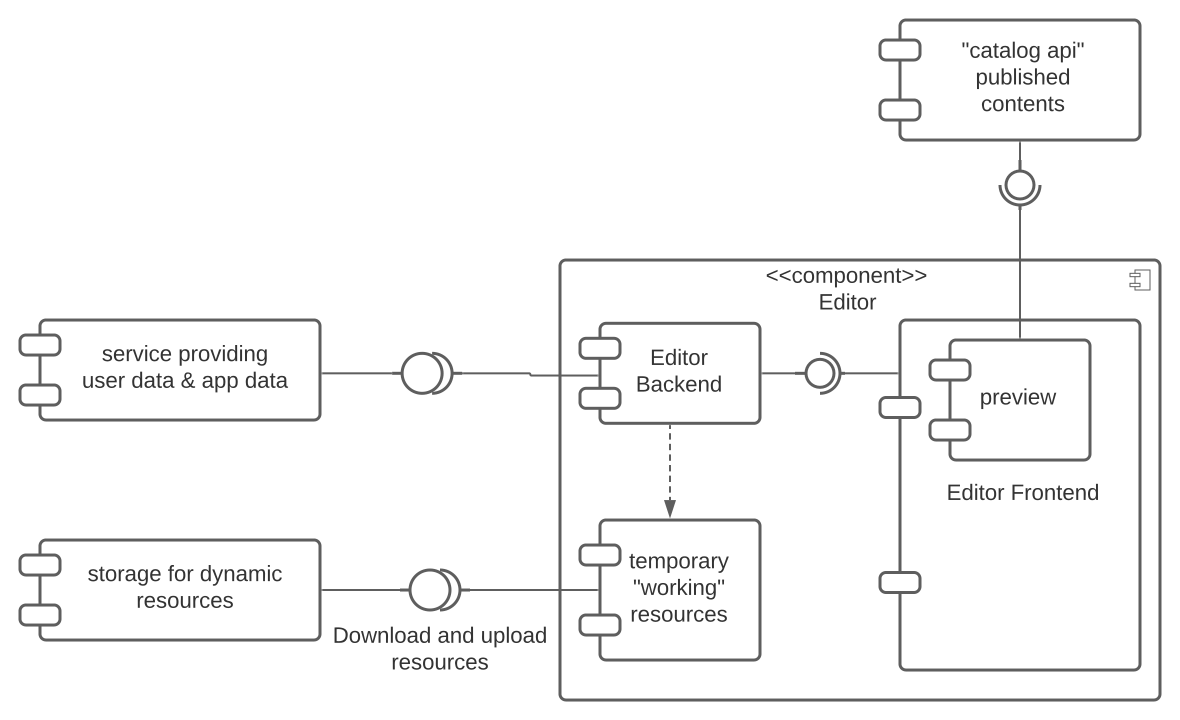
\includegraphics[width=0.7\textwidth]{pics/editor_uml_component.png}
  \caption[]{UML component diagram of the integration into the exisitng environment}
\end{figure}



\subsection{Evaluation}
\label{subsec:evaluation}

The evaluation towards the end of the thesis consists of using some of the methods mentioned above a last time. There the focus will probably be on a survey and evaluating analytics data, as well as getting verbal feedback from test users.
The results then get compared to the results raised earlier to identify improvements in the productivity of the users.

From that results, more abstract realizations about developing new software with HCI methods in constrained exisitng environments can be elaborated.
